\section{GraalVM}\label{chapter:graalvm}

Ważnym obszarem badań nad optymalizacją Javy i jej użycia w AWS Lambda, są technologie pozwalające na zmianę sposobu kompilacji i uruchamiana aplikacji.
Jedną z technologii, które zyskusje na popularności w tym zakresie, jest GraalVM.
Jest to możliwe m.in. dzięki użyciu kompilatora JIT (ang. Just-In-Time) w połączeniu z kompilacją AOT (ang. Ahead-Of-Time) \cite{8756917}.
GraalVM oferuje zaawansowaną architekturę pozwalającą na kompilację i uruchomienie aplikacji w postaci obrazów natywnych.
Stanowi to alternatywę dla klasycznej maszyny wirtualnej Javy, a dodatkowo skupia się na jej wydajności.
Poniższy podrozdział poświęcono analizie działania omawianego rozwiązania, jego zalet i słabych stron.

Kluczowym mechanizmem GraalVM jest kompilacja AOT (ang. Ahead-Of-Time) do postaci tzw. obrazów natywnych (ang. native images) \cite{8756917}.
Ma to bezpośredni wpływ na wydajność działania aplikacji.
W modelu tradycyjnym, kod bajtowy Java jest interpretowany i kompilowany dynamicznie przez maszynę wirtualną w trakcie działania aplikacji.
Podejście AOT przenosi znaczną część z tych operacji na etap budowania artefaktu. 
Istotnym elementem tego procesu jest agresywna, statyczna analiza kodu \cite{9245290}, w celu identyfikacji osiągalnych w trakcie działania części.
Pozwala to na odrzucenie nieużywanych fragmentów kodu (np. z używanych bibliotek), co pozwala na zmniejszenie wielkości obrazu natywnego.
Aspekt ten może być kluczowy w kontekście AWS Lambda, ze względu na wpływ wielkości artefaktu na wydajność \cite{8116416}.
Po analizie kodu, dokonywana jest inicjalizacja klas, a stan aplikacji, w tym częściowo zainicjalizowana sterta, jest utrwalany.
W celu lepszej optymalizacji, operacje te są powtarzane, co zostało przedstawione na Rysunku \ref{fig:graalvm_build_process}.

Jako wynik kompilacji powstaje samodzielny, zoptymalizowany plik binarny.
Nie wymaga on do uruchomienia pełnej maszyny wirtualnej Java, a jedynie minimalnego środowiska wykonawczego dostarczanego przez SubstrateVM, będącego częścią GraalVM \cite{8756917}.
Różnica ta ma fundamentalne znaczenie w kontekście wydajności AWS Lambda.
Eliminowana jest konieczność wykonywania czasochłonnych operacji typowych dla startu tradycyjnej maszyny wirtualnej Java, takich jak ładowanie klas czy jej inicjalizacja.
Wszystkie te zadania zostały już wykonane wcześniej, w procesie budowy obrazu natywnego.
Dzięki temu tworzona przez programistę funkcja AWS Lambda nie będzie operować w zarządzanym środowisku Java.
Zamiast tego, usługi muszą opierać się o niestandardowe środowiska wykonawcze, oferujące wyłącznie system operacyjny (Amazon Linux 2023 lub Amazon Linux 2) \cite{awsLambdaDeveloperGuide}.
Ich użycie pozwala także na realizację drugiej zalety GraalVM, czyli redukcji zapotrzebowania na pamięć operacyjną \cite{9245290}.

Pomimo pozytywnego wpływu na wydajność, zastosowanie kompilacji AOT w GraalVM wiąże się także z ograniczeniami.
Jednym z nich jest obsługa dynamicznych cech Javy, takich jak refleksja (ang. reflection), dynamiczne proxy, serializacja czy natywny interfejs Java (JNI)
Wynika to z faktu użycia agresywnej statycznej analizy kodu.
Napotyka ona trudności w przewidzeniu wszystkich dynamicznie ładowanych klas, pól i metod, które nie są jawnie osiągalne w kodzie źródłowym.
Problem ten wymaga użycia dodatkowych mechanizmów GraalVM \cite{graalvm-reflection-jdk21}.
Polegają one na przygotowaniu dodatkowych metadanych dla klas, co wymaga jednak dodatkowej obsługi.

\begin{figure}
    \centering
    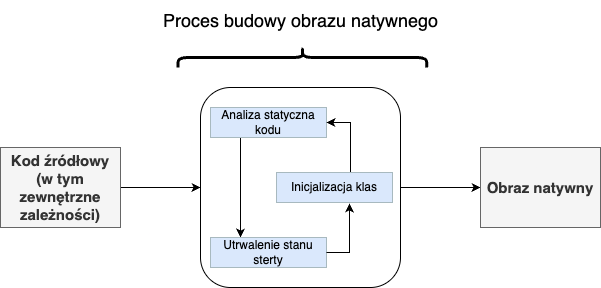
\includegraphics[width=0.95\textwidth]{charts/graalvm-build-process.drawio.png}
    \caption{Uproszczony proces budowy obrazu natywnego GraalVM [źródło:~opracowanie~własne]}
    \label{fig:graalvm_build_process}
\end{figure}

Kolejnym aspektem, który może negatywnie wpłynąć na rozwój oprogramowania przy użyciu GraalVM, jest czasochłonność procesu kompilacji.
Generowanie w pełni zoptymalizowanego obrazu natywnego jest operacją bardziej złożoną niż standardowa kompilacja kodu Javy do postaci bajtowej.
W praktyce oznacza to, że proces budowania artefaktu dla funkcji AWS Lambda może trwać odczuwalnie dłużej.
Może mieć to znaczący wpływ na rozwój oprogramowania, szczególnie w przypadku częstych iteracji i tworzenia nowych wersji funkcji.
Dłuższy czas kompilacji może także wpłynąć na ogólną efektywność procesów ciągłej integracji i ciągłego dostarczania (ang. CI/CD).

Jednym z sposobów poprawy doświadczeń programistów przy pracy z GraalVM, jest użycie odpowiednich frameworków.
Jednym z nich jest Quarkus \cite{9245290}, który został zaprojektowany z myślą o środowiskach chmurowych.
Kluczową cechą Quarkusa jest przeniesienie jak największej liczby operacji inicjalizacyjnych i konfiguracyjnych na etap budowania aplikacji.
Obejmuje to między innymi wstrzykiwanie zależności, przetwarzanie adnotacji oraz konfigurację rozszerzeń. 
Dzięki temu, w czasie budowania obrazu natywnego, Quarkus jest w stanie przeprowadzić szczegółową analizę aplikacji.
Poprzez użycie odpowiednich annotacji pozwala on na oznaczenie klas niezbędnych dla mechanizmów refleksji czy proxy \cite{quarkus-docs}.
Dzięki temu jest on w stanie automatycznie wygenerować niezbędne metadane dla klas.
Dane te następnie pozwalają na użycie wspomnianych mechanizmów w GraalVM.
Innymi, konkurencyjnymi do Quarkusa frameworkami, które oferują wsparcie dla obrazów natywnych są Helidon i Micronaut \cite{9245290}.
Ich popularność wskazuje na wysokie zainteresowanie takimi technologiami w społeczności programistów Java, dlatego jest to interesujący kierunek rozwoju dla funkcji AWS Lambda.
